% Setup -------------------------------

\documentclass[a4paper]{report}
\usepackage[a4paper, total={6in, 10in}]{geometry}
\setcounter{secnumdepth}{3}
\setcounter{tocdepth}{3}

\usepackage{hyperref}

% Images package
\usepackage{graphicx}

% Encoding
%--------------------------------------
\usepackage[T1]{fontenc}
\usepackage[utf8]{inputenc}
%--------------------------------------

% Portuguese-specific commands
%--------------------------------------
\usepackage[portuguese]{babel}
%--------------------------------------

% Hyphenation rules
%--------------------------------------
\usepackage{hyphenat}
%--------------------------------------

% Capa do relatório

\title{
	Computação Avançada
	\\ \Large{\textbf{Projeto de Avaliação}}
	\\ -
	\\ Mestrado em Engenharia Informática
	\\ \large{Universidade do Minho}
	\\ Relatório
}
\author{
	\begin{tabular}{ll}
		\textbf{Grupo}
		\\\hline
		PG41081 & José Alberto Martins Boticas
		\\
		PG41090 & João Ribeiro Imperadeiro
		\\
		PG41091 & Nelson José Dias Teixeira
	\end{tabular}
}

\date{\today}

\begin{document}

\begin{titlepage}
    \maketitle
\end{titlepage}

% Resumo

\begin{abstract}
	Este projeto de avaliação relativo à unidade curricular de Computação Avançada consiste, globalmente, em instalar e configurar um \textit{cluster} de \textit{HTCondor} 
	com pelo 3 nós e utilizar o mesmo na resolução de uma tarefa de processamento (compressão de um vídeo, em \textit{mp4}).
\end{abstract}

% Índice

\tableofcontents

% Introdução

\chapter{Introdução} \label{intro}
\large{
	De forma sucinta, neste trabalho prático é pedida a implementação de um \textit{cluster} \textit{HTCondor} para a realização de tarefas de processamento de grandes volumes de 
	dados ou de elevada complexidade. Para além disso, como seria de esperar, é necessário especificar o sistema desenvolvido pelos elementos deste grupo bem como aspetos adicionais 
	associados ao mesmo.
	
	Neste caso em concreto, é pedido algo mais específico, isto é, o desenvolvimento de uma aplicação de \textit{resizing} de video. Através deste caso, é possível mostrar o funcionamento 
	do \textit{cluster} em questão, transformando, por exemplo, um determinado video com resolução \textit{fullHD} (1080p) na resolução \textit{SD} (720p).

	A correta realização desta tarefa passa por reduzir o tempo necessário à conversão do video em causa. Como tal, é possível partir o video original em vários segmentos, fazendo a conversão 
	de cada um destes e, no fim, juntá-los todos no video de resultado. Seguindo a sugestão do docente desta unidade curricular, foi utilizado o comando \textit{ffmpeg} para auxiliar a 
	execução deste tipo de tarefa.
}

\chapter{Implementação}

    \section{Instalação e configuração do cluster}
	% Falar dos 3 nós; configuração de uma máquina master e duas workers; ...
	
	\begin{figure}[h]
		\centering
		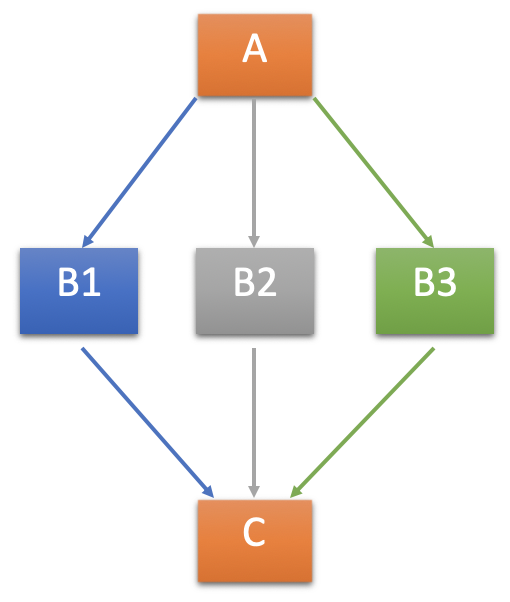
\includegraphics[scale=0.5]{Arquitetura-HTCondor.png}
		\caption{Arquitetura do sistema \textit{HTCondor}}
		\label{}
	\end{figure}
    
    \section{Realização da tarefa}
    % Explicar os scripts

\chapter{Conclusão}
\large{

}

\chapter{Webgrafia}
    \begin{itemize}
        \item Documentação - \textbf{\textit{ffmpeg}}:
        \par \textit{\url{https://www.ffmpeg.org/ffmpeg.html}}
    \end{itemize}

\appendix
\chapter{Observações}

\end{document}
